\section{РЕАЛИЗАЦИЯ CLASS-BASED WFQ В ЯДРЕ LINUX}

	\subsection{Описание устройства подсистемы планировки в ядре Linux}
	% Информация из комментариев к ним.
	% Файлы: linux/net/sched/sch_api.c, linux/include/net/{sch_generic.h,pkt_sched.h}. 

	В операционной системе Linux
	дисциплина обслуживания, обозначемая термином qdisc, используется
	для выбора пакетов из выходящей очереди для отправки на выходной интерфейс.
	Схема движения пакета приведена на Рисунке~\ref{pic:flow}. Выходная очередь
	обозначена термином egress; именно на этом этапе следования пакета
	и работает механизм qdisc.\cite{lartc}

    \begin{figure}[ht!]
        \center
        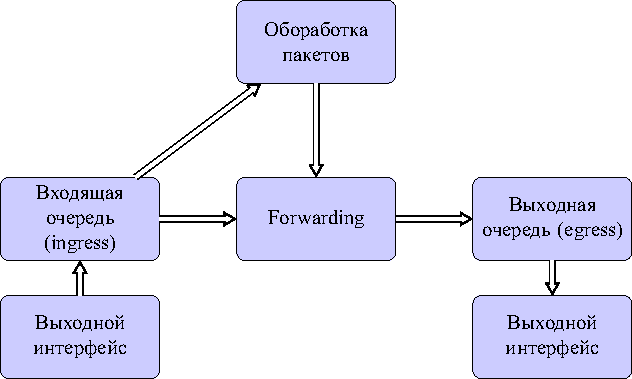
\includegraphics{pdfimages/qdisc.pdf}
        \caption{Схема движения пакета в системе Linux\cite{tcpip}}
		\label{pic:flow}
    \end{figure}

	В ощем случае, дисциплина обслуживания -- это чёрный ящик, который может
	ставить пакеты в очереди и вынимать их из очереди, когда устройство
	готово к отправке, в порядка и во время, определёнными спрятанным в ящике
	алгоритмом. В ядре Linux дисциплины обслуживания представляются в качестве
	модулей ядра, которые реализуют предоставляемый ядром интерфейс.

	Linux поддерживает классовые и бесклассовые дисцплины обслуживания. Примером
	бесклассовой дисциплины служит pfifo\_fast, классовой -- htb.\cite{lartc}

	Классы представляют собой одельные сущности в иерархии основной дисциплины.
	Если структура представляет собой дерево, то в классах-узлах могут содержаться
	фильтры, которые определят пакет в нужный класс-потомок. В классах-листьях
	непосредстенно располагаются очереди, которые управляются внутренней дисциплной
	обслуживания (обычно это pfifo\_fast). 

	Каждый интерфейс имеет корневую дисцплину (по умолчанию pfast\_fifo), которой
	назначается идентификатор (handle), который используется для обращения к дисциплине.
	Этот идентификатор состоит из двух частей: мажорной (MAJ) и минорной (MIN); мажорная
	часть определяет родителя, минорная -- непосредственно класс. На Рисунке~\ref{pic:clheirh}
	представлен пример иерархии, основанной на описанных идентификаторов.

	\begin{figure}[ht!]
		\centering
		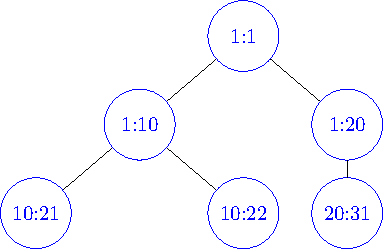
\includegraphics{./pdfimages/class_hierh.pdf}
		\caption{Схема классовой иерархии с использованием идентификаторов MAJ:MIN}
		\label{pic:clheirh}
	\end{figure}

	Такая иерархия позволяет организовать гибкую систему классификации с набором классов
	и их подклассов, пакеты в которые назначются фильтрами, которые предоставляются ядром.

	CBWFQ является классовой дисциплиной обслуживания с конфигурируемыми классами (в отличие от
	дисциплины PQ) и классом по умолчанию. Ядро предоставляет ряд полезных функций и структур
	данных, которые значительно упрощают написания необходимого кода в ядре и избавляет от
	совершения ряда критических ошибок. Таким образом, для наиболее эффективной реализации
	дисципилны обслуживания CBWFQ следует использовать предоставляемые ядром функции.

	\subsection{Интерфейс управления трафиком}

	В Linux управление трафиком осуществляется с помощью подсистемы Traffic Control,
	которая предоставляет пользовательский интерфейс с помощью утилиты \texttt{tc}.
	\texttt{tc} -- это пользовательская программа, которая позволяет настраивать
	дисцплины обслуживания в Linux. Она использует Netlink в качестве
	коммуникационного канала для взаимодействия между пользовательским
	пространством и пространством ядра. \texttt{tc} добавляет новые дисциплины
	обслуживания, классы трафика, фильтры и предоставляет команды для
	управление всеми обозначенными объектами.\cite{tcpip}

	\texttt{tc} предоставляет интерфейс для дисцплины обслуживания,
	представленный структурой \lstinline{struct qdisc_util}, которая
	описывает функции для отправления команд и соответствующих параметров ядру
	и вывода сообщений о настройки дисциплины, списках классов и их настройки, а
	также статистику от ядра. Сообщение, помимо общей информации для подсистемы,
	содержит специфичную для дисциплины структуру с опциями, описываемую
	в заголовке ядра (pkt\_sched.h). 

	Для назначения новой дисциплины обслуживания на интерфейс используется
	команда \lstinline{tc qdisc add} системными параметрами (к примеру, название
	интерфейса), названием дисциплины и её локальными параметрами, которые
	определяются и обрабатываются в модуле дисциплины для утилиты \texttt{tc}. 
	Для внесения измнений и удаления используются соответственно \lstinline{tc change}
	и \lstinline{tc delete}.

	Для классовых дисциплин используется команда \lstinline{tc class} с подкомандами
	\lstinline{add}, \lstinline{change} и так далее. Классы обычно имеют параметры,
	отличные от параметров всей дисциплины обслуживания, поэтому нуждаются в отдельной
	структуре данных и функции обработчике.


	Таком образом, для использования дисциплины обслуживания необходимо
	реализовать интерфейс в системе \texttt{tc}. Патчи для утилиты \texttt{tc}
	и ядра Linux, обеспечивающие взаимодействие между пользовательским пространством
	и дисциплиной представлен в Приложении А. 

	\subsection{Описание интерфейса}

	API ядра для подсистемы qdisc предосавтляет две функции: \lstinline{register_qdisc(struct Qdisc_ops *ops)}
	и обратную -- \lstinline{unregister_qdisc(struct Qdisc_ops *ops)}, которые регистрируют
	и разрегистрируют дисциплину обслуживания на интерфейсе. Важно отметить, что обе эти
	функции принимают в качестве аргумента структуру \lstinline{struct Qdisc_ops},
	которая явным образом идентифицирует дисциплину обслуживания в ядре.[Исходный код]

	Структура \lstinline{struct Qdisc_ops} помимо метаинформации содержит указатели на функции,
	которые должен реализовывать модуль дисциплины обслуживания для работы в ядре.[Исходный код]

	Поля этой структуры представляют собой указатели на функции с сигнатурой,
	представленной ниже[Исходный код].
	\begin{itemize}
		\item \lstinline{enqueue}\\
   		    \lstinline{int enqueue(struct sk_buff *skb, struct Qdisc *sch, struct sk_buff **to_free);} \\
			Фукнкция добавляет пакет в очередь. Если пакет был отброшен, функция
			возращает код ошибки, говорящий о том, был отброшен пришедший пакет или
			иной, чьё место занял новый.
		\item \lstinline{dequeue}\\
			\lstinline{struct sk_buff *dequeue(struct Qdisc * sch);} \\
			Функция, возвращающая пакет из очереди на отправку. Дисциплина
			может не передавать пакет при вызове этой функции по решению
			алгоритма, в таком случае вернув нулевой указатель; 
			однако то же значение алгоритм возвращает в случае, если очередь
			пуста, поэтому в таком случае дополнительно проверяется длина
			очереди.
		\item \lstinline{peek}\\
			\lstinline{struct sk_buff *peek(struct Qdisc * sch);}\\
			Функция возвращает пакет из очереди на отправку, не удаляя его из реальной очереди,
			как это делает функция \lstinline{dequeue}.
		\item \lstinline{init}\\
			  \lstinline{int init(struct Qdisc *sch, struct nlattr *arg);}\\
			  Функция инициализирует вновь созданный экземпляр дисциплины обслуживания \texttt{sch}.
			  Вторым аргументом функции является конфигурация дисциплины обслуживния, передаваемая
			  в ядро с помощью подсистемы Netlink.
		\item \lstinline{change}\\
			  \lstinline{int change(struct Qdisc *sch, struct nlattr *arg);}\\
			  Функция изменяет текущие настройки дисциплины обслуживания. 
		\item \lstinline{dump}\\
			  \lstinline{int dump(struct Qdisc *sch, struct sk_buff *skb);}\\
			  Функция отправляет по Netlink статистику дисциплины обслуживания.
	\end{itemize}

	Также структура содержит указатель на другую структуру \lstinline{struct Qdisc_class_ops},
	которая описывает указатели функции исключительно для классовых дисциплин.
	Ниже приведены наиболее важные сигнатуры и их описания.[Исходный код]
	\begin{itemize}
		\item \lstinline{find}\\
			\lstinline{unsinged long find(struct Qdisc *sch, u32 classid);}\\
			Функция возвращает приведённый к \lstinline{unsinged long} адресс класса по его идентификатору (\lstinline{classid}).
		\item \lstinline{change} \\
			\lstinline{int change(struct Qdisc *sch, u32 classid, u32 parentid, struct nlattr *attr, unsinged long *arg);}
			Функция используется для изменения и добавления новых классов в иерархии классов. 
		\item \lstinline{tcf_block}, \lstinline{bind_tcf}, \lstinline{unbind_tcf}\\
			В данном случае, описание сигнатур не даст какой-либо значимой информации; практически
			для всех дисциплин обслуживания они идентичны. Эти функции предназначаются для работы
			системы фильтрации.
		\item \lstinline{dump_class}\\
			\lstinline{int dump_class(struct Qdisc *sch, unsinged long cl, struct sk_buff *skb, struct tcmsg *tcm);} \\
			Функция предназначается для передачи по Netlink информации о классе и дополнительной статистики, собранной
			во время функционирования класса.
	\end{itemize}

	Для классовых дисцплин, помимо описанного, реализуют классификацию пакетов, которая
	определяет класс, куда попадёт пакет. Классификация обычно выражается в функции \lstinline{classify},
	которая определяет, какому классу принадлежит пакет, и возвращает указатель на этот класс.
	Экземпляр структур для дисциплины обслуживания CBWFQ приведён в патче, представленном в Приложении B.

	\subsection{Алгоритм CBWFQ}

		\subsubsection{Структура хранения данных Class-Based WFQ}

	
			Определение структуры представлено в Приложении B. 

		\subsubsection{Вычисление виртуального времени}
			\begin{algorithmic}
				\Function{eval\_finish\_time}{Q, c, pkt}
					\If {c.queue is not empty}
        				\State {// Виртуальное время }
        				\State v $\gets$ \Call{V}{pkt.arrival\_time}
        				\State {// Вычисление времени начала обработки.}
        				\State s $\gets$ \Call{max}{c.prev\_ft, v} 
					\Else
						\State s $\gets$ 0
					\EndIf
    				\State {// В ядре вычисления с плавающей запятой затруднены,}
    				\State {// из-за чего стараемся изменить вычисления так, чтобы их избегать.}
    				\State f $\gets$ s $ + \dfrac {\text{pkt.len} \cdot \text{Q.bandwidth}} {\text{q.rate}}$
				\EndFunction
			\end{algorithmic}

		\subsubsection{Добавление пакета в очередь}

			Алгоритм добавления пакета обычно состоит из схожих действий:
			классификация и добавление в очередь, если есть место в очереди
			для пакета. 

			\begin{algorithmic}
				\Function{enqueue}{Q, pkt}
					\State {// Сначала нужно классифицировать пакет в очередь.}
					\State {// Функция классификации определяет очередь, которой}
					\State {// соответствует пакет, с помощью заданных фильтров}
					\State {// и возвращает указатель на класс.}
					\State c $\gets $ \Call{classify}{Q, pkt}
					\If {\Call{q.enqueue}{pkt}}
    					\State {// Ради экономии ресурсов, храним два виртуальных времени:}
    					\State {// текущего и прошлого пакета; и считаем время только для}
    					\State {// пакета, который пришёл в пустую очередь}
    					\If {c.queue is empty}
							\State c.prev\_ft $\gets$ c.ft
							\State c.ft $\gets$ \Call{eval\_finish\_time} {Q, c, pkt}
    					\EndIf
					\EndIf
				\EndFunction
			\end{algorithmic}

			Специфичным добавлением CBWFQ является вычисление времени конца обработки.
			Оно вычисляется каждый раз, когда пакет добавляется в пустую очередь.
			Это сделано, чтобы не реализовывать дополнительные структуры для
			хранения и тем самым тратить меньше ресурсов.

		\subsubsection{Удаление пакета из очереди}

			\begin{algorithmic}
				\Function{dequeue}{Q}
					\State {// Находим класс с наименьшим финальным временем.}
					\State c $\gets$ \Call{find\_min\_ft}{Q}
					\State {// Вычисляем новое финальное время для следующего пакета}
					\State pkt\_next $\gets$ \Call{c.peek}{c.queue}
					\State c.ft $\gets$ \Call{eval\_finish\_time}{Q, c, pkt\_next}
					\State \Return \Call{dequeue}{c.queue}
				\EndFunction
			\end{algorithmic}

	\subsection{Тестирование модуля}

		Для тестирования модуля ядра была создана система виртуальных машин на основе
		системы эмуляции программного обеспечения QEMU. Схема тестовой среды представлена
		на Рисунке~\ref{pic:testscheme}. Источником служит узел, от которого исходит трафик;
		траблицы маршрутизации настроены таким образом, чтобы весь трафик, который
		должен попасть на узел-цель шёл через промежуточный узел, на котором
		настроена тестируемая дисциплина обслуживания CBWFQ.

        \begin{figure}[ht!]
        	\center
        	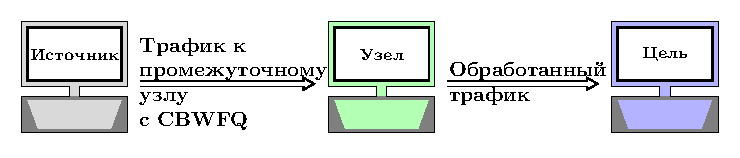
\includegraphics[scale=1.2]{pdfimages/test_scheme.pdf}
        	\caption{Схема тестовой среды.}
			\label{pic:testscheme}
        \end{figure}

		В Листинге~\ref{lst:tccmd} приведена система настройки дисциплины на промежуточном узле.
		Переменные окружения \lstinline{TESTPORT1} и \lstinline{TESTPORT2} содержат в себе
		номера портов, на которые направлен трафик (номера портов меняются). При добавлении
		дисципилны на интерфейс необходимо указать пропускную способность канала для
		корректных расчётов полосы пропускания для классов. При конфигурации классов
		во второй и третьей сторках происходит назначение каждому классу доли
		пропускной способности от канала в процентах (так же возможно указать точное
		количество пропускной способности в bps). В четвёртой и пятой строках
		происходит назначение фильтров, которые фактически определяют трафик
		для класса. На один класс можно назначить множество фильтров, посему
		это задача пользователя корректно определить трафик класса. 

        \begin{figure}[ht!]
    		\center
    		\begin{lstlisting}[frame=lines,
    						  caption={Список команд для конфигурации дисциплины обслуживания CBWFQ.},
    						  label={lst:tccmd},
    						  style=tcstyle]
tc qdisc add dev eth1 cbwfq bandwidth 10
tc class add dev eth1 parent 1: classid 1:2 cbwfq rate 80 percent 
tc filter add dev eth1 parent 1: protocol ip u32 match ip sport $TESTPORT flowid 1:2
    		\end{lstlisting}
        \end{figure}

		Для тестирования пропускной способности, которая была выделена каждому классу,
		была использована утилита iperf версии 3, которая запускалась на узле-источнике (Листинг~\ref{lst:iperfsrc}) и
		узле-цели (Листинг~\ref{lst:iperfdst}). По умолчанию iperf генерирует TCP-трафик c окном,
		указаным в командной строке на стороне сервера; с клиента на сервер передаётся трафик в три потока.

        \begin{figure}[ht!]
    		\center
    		\begin{lstlisting}[frame=lines,
    						  caption={Команда iperf на узле-источнике (клиентская сторона).},
    						  label={lst:iperfsrc}]
iperf3 -c $SERVERIP --cport $TESTPORT -P 2
    		\end{lstlisting}
        \end{figure}	

        \begin{figure}[ht!]
    		\center
    		\begin{lstlisting}[frame=lines,
    						  caption={Команда iperf на узле-цели (серверная сторона).},
    						  label={lst:iperfdst}]
iperf3 -s --logfile "$EXPNUM".log
    		\end{lstlisting}
        \end{figure}

		iperf выводит информацию о пропускной способности канала. 

		Для указанной в Листинге~\ref{lst:tccmd}
		конфигурации после серии тестов были получены результаты, отображённые на Рисунке~\ref{pic:plot}.

        \begin{figure}[ht!]
        	\center
        	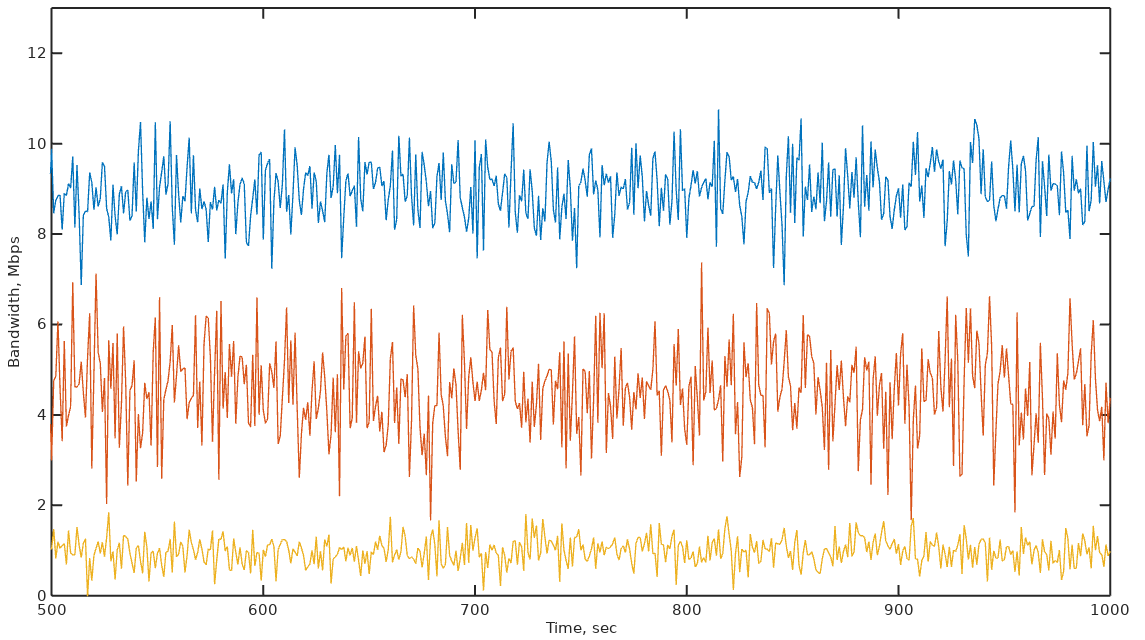
\includegraphics[width=1.1\linewidth]{pdfimages/plot.pdf}
        	\caption{График распределения процента пропускной способности (ПС) по типам трафика в течение времени.}
			\label{pic:plot}
        \end{figure}
